% !TEX program = xelatex
\documentclass[12pt,a4paper]{ctexart}
\usepackage[top=2.6cm,bottom=2.6cm,left=2.9cm,right=2.9cm]{geometry}
\usepackage{setspace}
\usepackage{graphicx}
\usepackage{caption}
\captionsetup{font={small},labelsep=space}
\onehalfspacing

\begin{document}
\thispagestyle{empty}
\begin{center}
{\LARGE\heiti 第八届中国研究生人工智能创新大赛}\\[0.5cm]
{\zihao{3}\heiti 参\,赛\,作\,品\,简\,介}\\[1.2cm]
\renewcommand{\arraystretch}{1.5}
\begin{tabular}{rl}
{\zihao{4} 项目名称：} & {\zihao{4} 知识超图驱动的复杂学术查询智能搜索系统（ScholarGraph）}\\
{\zihao{4} 团队名称：} & {\zihao{4} Dong}\\
\end{tabular}
\end{center}
\vspace{1.2cm}

\noindent ScholarGraph 是知识超图驱动的复杂学术查询智能搜索系统。针对专家查询与关键词匹配的语义鸿沟，系统以自演化知识超图为底座融入检索全流程：查询理解用冻结 schema 解析意图生成实体查询；召回阶段增量建图、沿引用意图边定向探索文献；输出按方法演化链组织、逐条溯源至原文。官方基准 AutoScholarQuery 上 $F_1$@5 从 0.000 提升至 0.150（holdout 对照），为已发表 S2+LLM 基线的 34 倍；RealScholarQuery 首测不用 Google 达最强 Google 基线量级召回；SPARBench 单 API+LLM 形态第一。成本约为参考系统的 1/20，超图随使用生长。

\vspace{0.8cm}
{\small\noindent（正文 291 字，符合 300 字以内要求）}

\vspace{0.6cm}
\begin{figure}[htbp]
\centering
\begin{minipage}[t]{0.47\textwidth}\centering
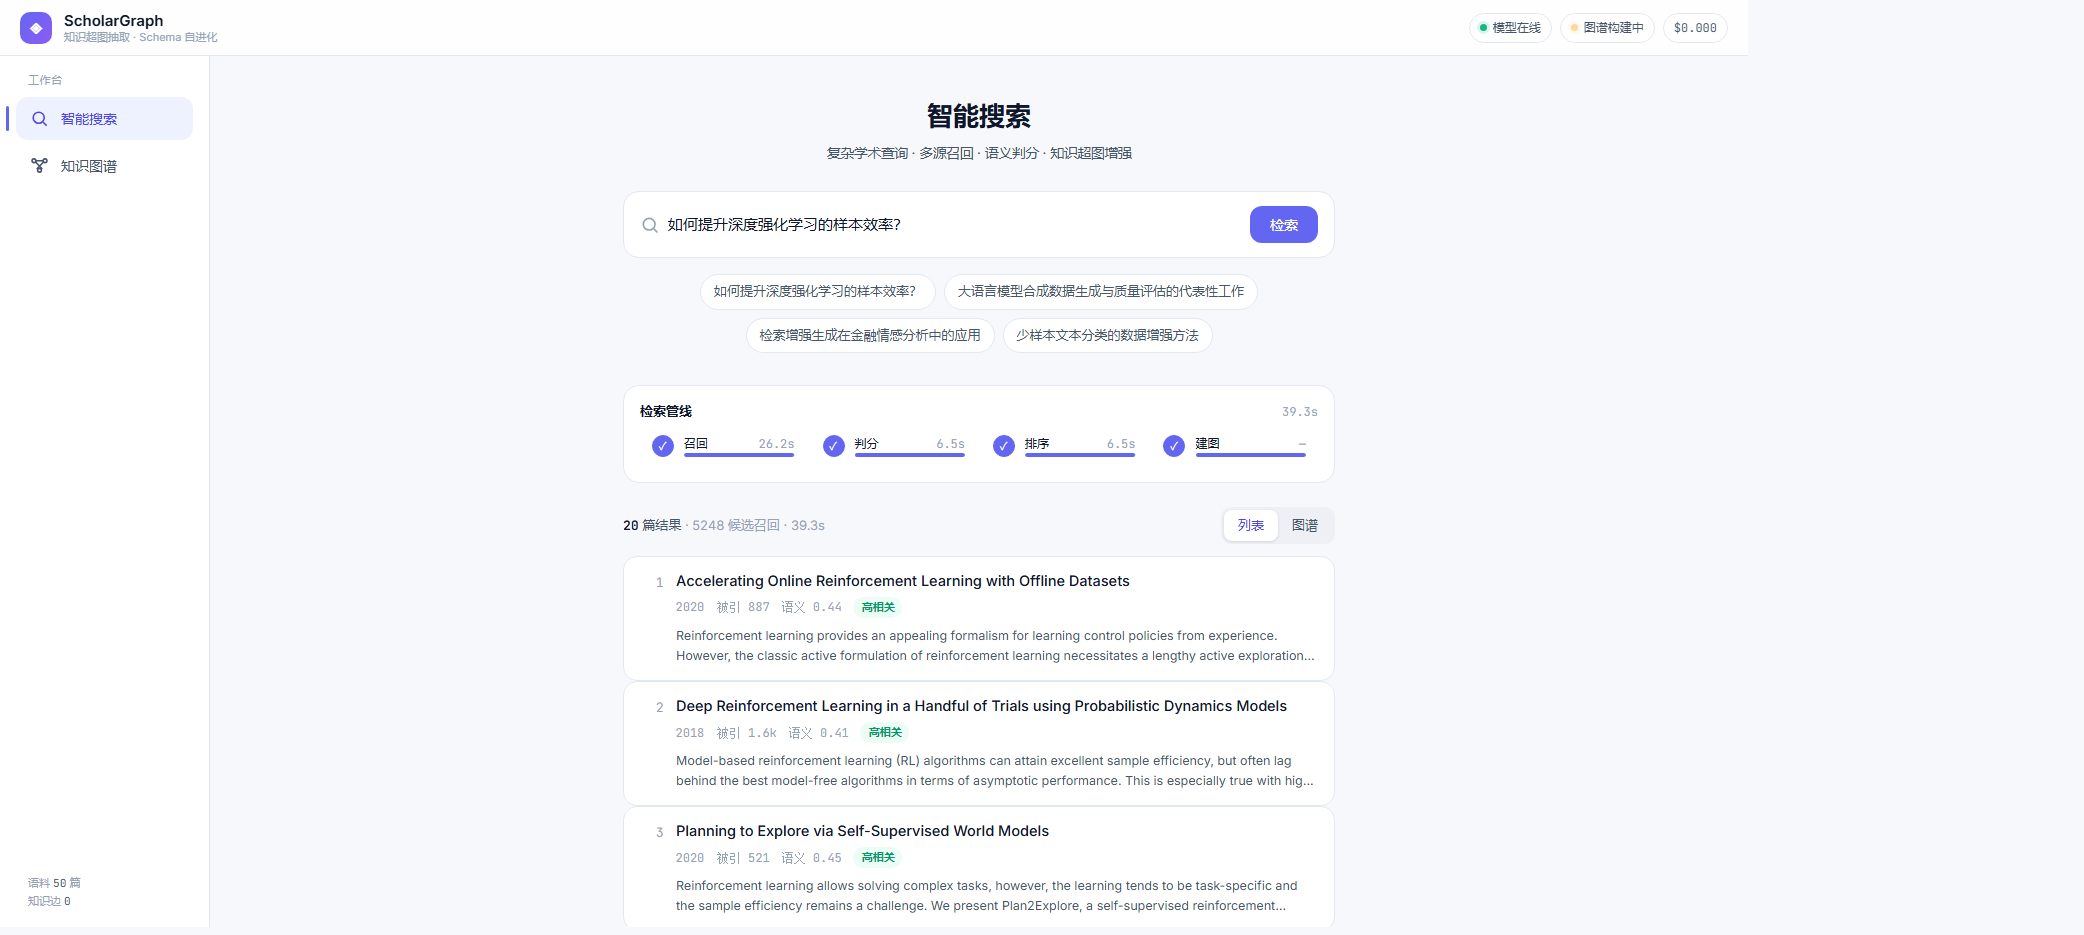
\includegraphics[width=\linewidth]{figs/search-results.png}\\[2pt]
{\footnotesize 搜索结果与管线阶段}
\end{minipage}\hfill
\begin{minipage}[t]{0.47\textwidth}\centering
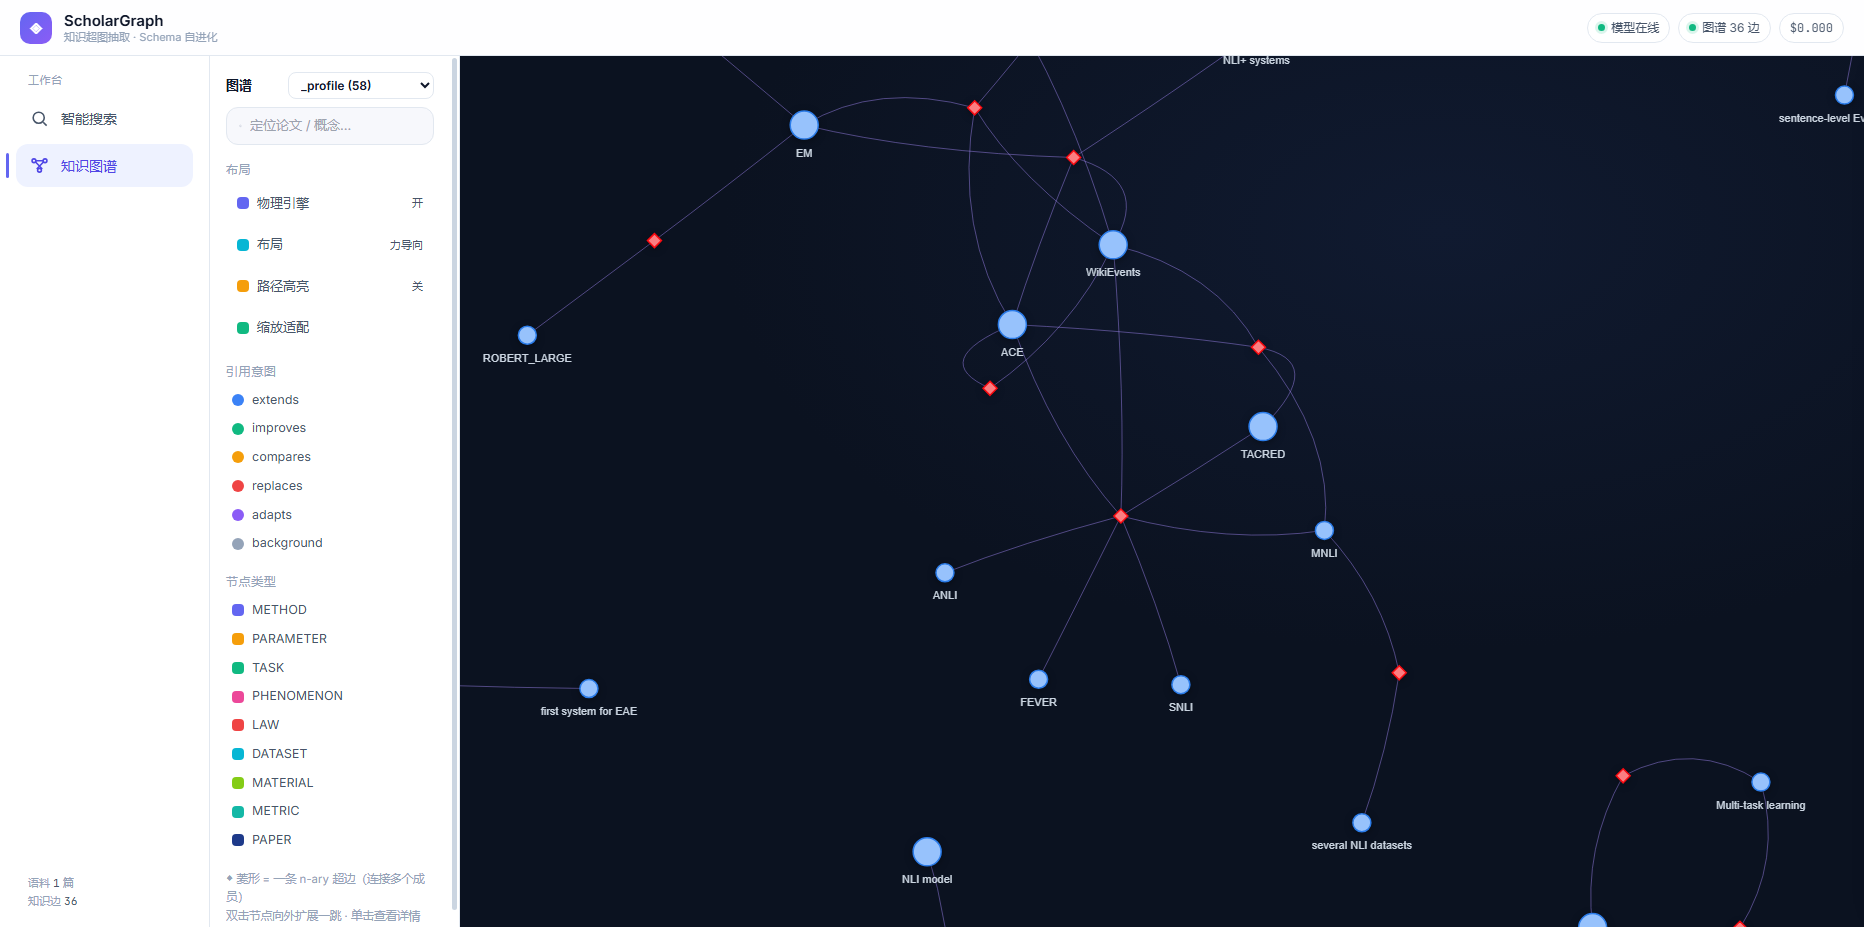
\includegraphics[width=\linewidth]{figs/contest_shot_graph_explorer_full.png}\\[2pt]
{\footnotesize 领域知识图全貌}
\end{minipage}

\vspace{0.6em}
\begin{minipage}[t]{0.47\textwidth}\centering
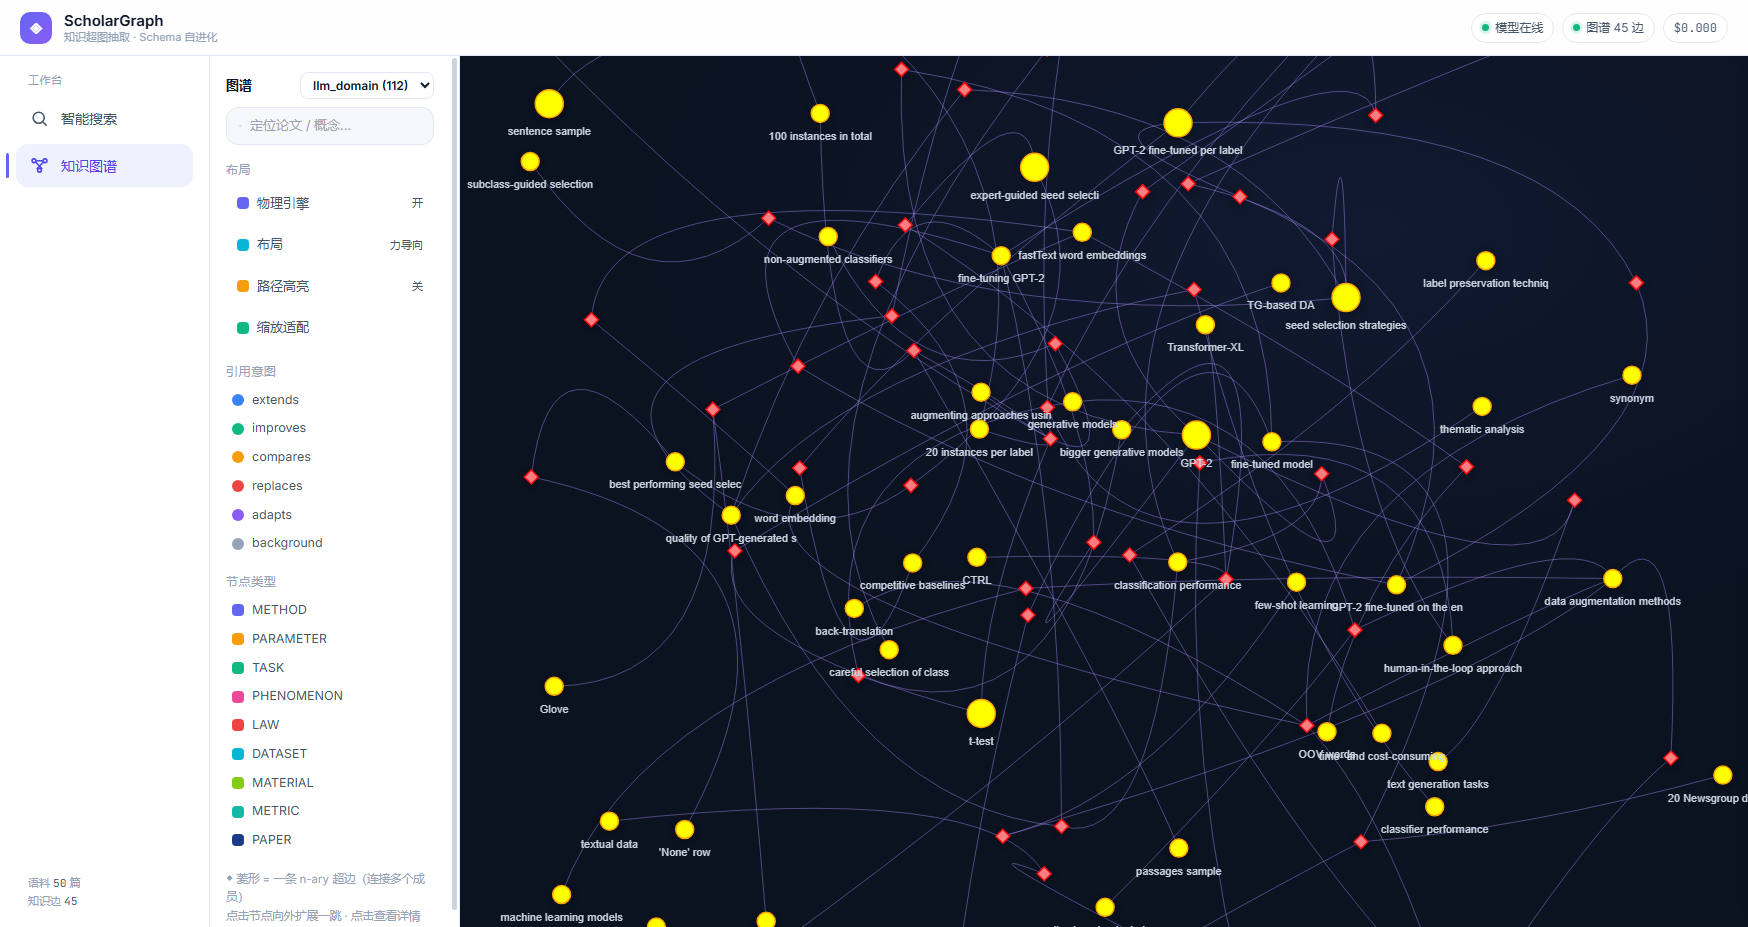
\includegraphics[width=\linewidth]{figs/graph-with-hubs.png}\\[2pt]
{\footnotesize 超边枢纽与引用意图着色}
\end{minipage}\hfill
\begin{minipage}[t]{0.47\textwidth}\centering
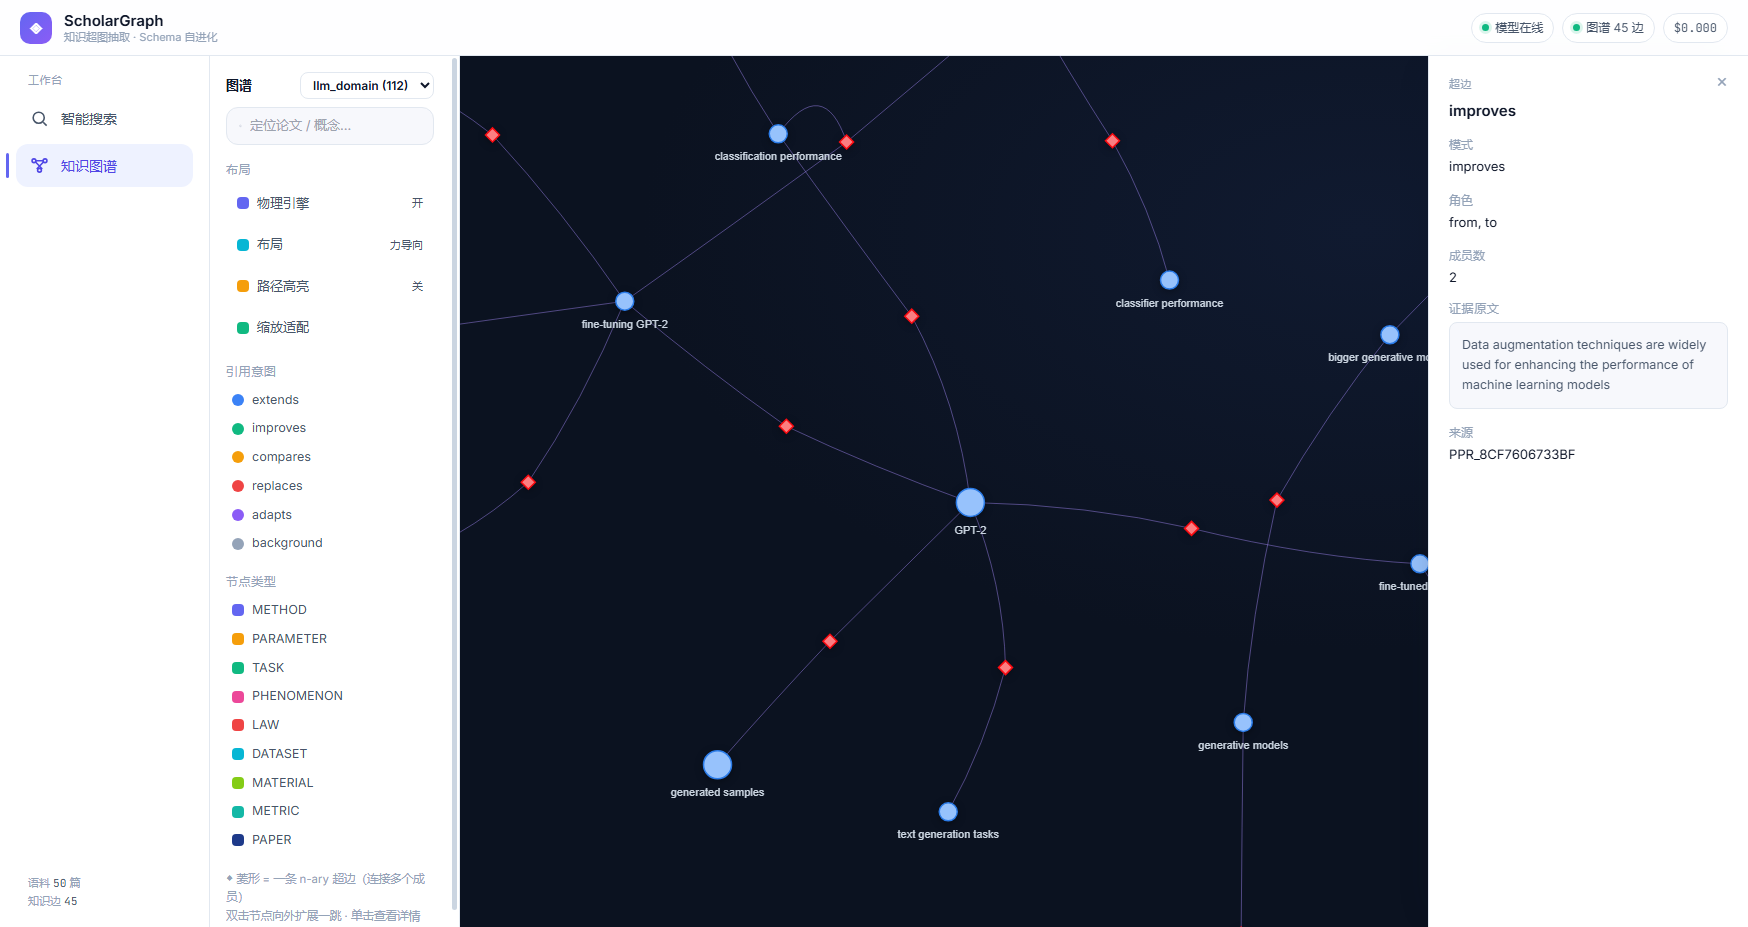
\includegraphics[width=\linewidth]{figs/provenance-drawer.png}\\[2pt]
{\footnotesize 逐条结论的证据溯源}
\end{minipage}
\caption{系统界面示意：检索、知识超图、引用意图与证据溯源}
\label{fig:intro}
\end{figure}

\end{document}
